\chapter{Problem statement}

%V této kapitole detailně popíšeme zadání problému, kterým se v této práci %zabýváme. Tento problém byl originálně zadán v kvalifikačním kole Google Hash %Code \cite{google_coding_competitions} 2021. Google Hash Code byla globální %týmová programovací soutěž, fungující mezi lety 2014--2022, kde týmy 2--4 %soutěžících řešily optimalizační úlohu s cílem dosáhnout co nejlepšího skóre v %omezeném čase 4 hodin.

In this chapter, we describe in detail the problem statement that we address in this thesis. This problem was originally assigned in the Google Hash Code \cite{google_coding_competitions} 2021 qualifying round. Google Hash Code was a global team programming competition, running between 2014--2022, where teams of 2--4 competitors solved an optimization problem with the goal of achieving the best score in a limited time of 4 hours.

%Klasický postup řešení vypadal následovně: načtění vstupních dat, vytvoření triviálního řešení a jeho zapsání do výstupního souboru v zadaném formátu, a nahrání řešení do vyhodnocovacího systému, kde bylo vidět nejen celkové skóre, ale také pár informačních statistik jako např. počet aut, které dorazily do cíle před deadlinem. U některých datasetů byla k dispozici i interaktivní vizualizace průběhu simulace, ze které bylo mimo jiné možné zjistit, jaká je struktura konkrétního datasetu. K odevzdání řešení tedy nebyl potřeba vlastní lokální simulátor, avšak ruční nahrávání řešení do vyhodnocovacího systému bylo pomalé a tedy nepoužitelné pro použití efektivních optimalizačních algoritmů.

The standard solution procedure was as follows: Read the input data, create a trivial solution and write it to the output file in the specified format, and upload the solution to the evaluation system, where you could see not only the total score, but also some informative statistics, such as the number of cars that reached the finish before the deadline. For some datasets, an interactive visualization of the simulation progress was also available, allowing to see the structure of a particular dataset. Although the local simulator was not needed to solve the problem, the manual upload of the solution to the evaluation system was slow and cumbersome and therefore not suitable for the use of efficient optimization algorithms.

%Většina týmů zvládla vytvořit triviální řešení, které se následně snažila náhodnými změnami hodnot zlepšovat. Ti nejlepší však dokázali napsat i vlástní simulátor a s jeho použitím  pustit více heuristik, díky kterým dosáhli lepšího skóre. I tak ale nebyl čas na nic lepšího než velmi jednoduché lokální prohledávání.

Most teams were able to construct trivial solutions, which they then tried to improve by randomly changing the values. However, the best teams were able to write their own local simulator and use it to run multiple heuristics to get better results. Still, there was no time for anything more complex than a very simple local search.

%Celkové skóre bylo součtem skór všech 6 datasetů ($a - f$). První dataset (a) sloužil jako "toy problem" --- byl dostatečně malý a dal se vyřešit na papíře. Je tedy třeba říct, že v každém datasetu \textit{nešlo} získat stejně bodů, a proto se soutěžící většinou zaměřili na datasety s největším možným ziskem bodů (d, f).

The total score was the sum of the scores of all 6 datasets (a -- f). The first dataset (a) served as a "toy problem" --- it was small enough to solve on paper. It should be said that distribution of points among different datasets was very unequal, so the contestants mostly focused on the datasets with the highest possible score (d, f) and skipped optimizing the rest (b, c, e).

\section{Problem description}

Nyní uvedeme detaily řešeného problému --- jeho kompletní zadání ze soutěže je dostupné v Google Coding Competitions archivu \footnote{\url{https://github.com/google/coding-competitions-archive/blob/main/hashcode/hashcode_2021_qualification_round.pdf}}. Ve zkratce, úloha zní takto: \textit{Mějme daný plán města, který popisuje ulice a křižovatky, a auta s přesně naplánovanými cestami městem. Cílem je nastavit semafory na křižovatkách tak, abychom minimalizovali celkový čas aut strávený při jízdě městem a aby co nejvíce aut dorazilo do cíle včas před zadaným deadlinem.}

Řečeno teorií grafů, plán města je \textit{orientovaný graf}, kde křižovatky jsou \textit{vrcholy} a ulice jsou \textit{orientované hrany} (Figure~\ref{fig:hashcode_city_plan} shows an example of such a city plan). Naplánovaná cesta pro každé auto je opravdu \textit{cesta} v tomto grafu --- má různý začátek a konec a žádná křižovatka se v ní neopakuje.

\begin{figure}
    \centering
    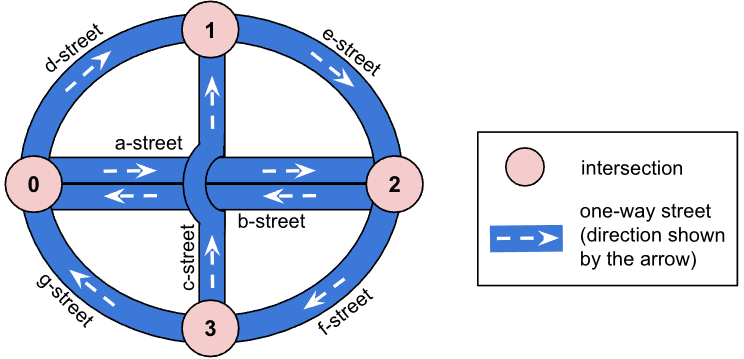
\includegraphics[width=\linewidth]{img/hashcode/figure1.png}
    %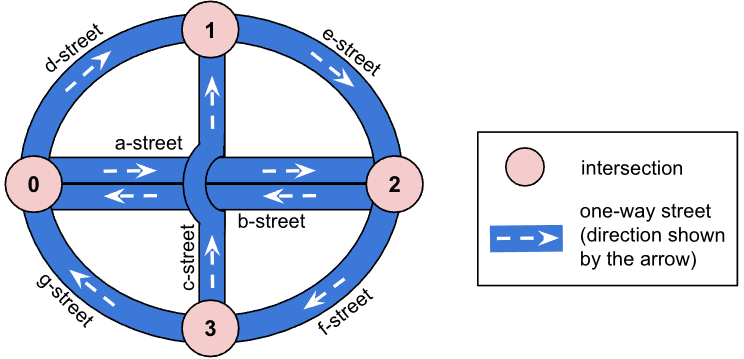
\includegraphics[width=.8\linewidth]{img/hashcode/figure1.png}
    \caption[Example of a city plan]{
        Example of a city plan \cite{google_coding_competitions}.
    }
    \label{fig:hashcode_city_plan}
\end{figure}

\subsection{Streets and intersections}
Ve městě máme množinu křižovatek
$I$, kde $2 \leq \abs{I} \leq 10^5$,
a množinu ulic 
$S \subseteq \{(u, v) | u,v \in I \land u \neq v\}$, kde $2 \leq \abs{S} \leq 10^5$.
Každá ulice $s \in S$ je tedy unikátní jednosměrné spojení mezi dvěma různými křižovatkami $u$, $v$; dvě samostatné ulice v opačných směrech mezi stejnými dvěma křižovatkami $(u, v)$, $(v, u)$ jsou povoleny. Každá ulice $s \in S$ má fixní čas $l(s) \in \mathbb{N}_+$, který trvá autu projet ulicí od začátku do konce, nezávisle na ostatních autech na ulici.
Každá křižovatka $i \in I$ má množinu příchozích ulic $S_i^+ \subset S$, kde $|S_i^+| \geq 1$, a množinu odchozích ulic $S_i^- \subset S$, kde $|S_i^-| \geq 1$; tedy každá křižovatka má alespoň jednu příchozí ulici a alespoň jednu odchozí ulici.

\subsection{Traffic lights and schedules}
V každé křižovatce $i \in I$ je na konci každé \textit{příchozí} ulice $s^+ \in S_i^+$ semafor, který má dva stavy --- zelenou a červenou. Zelená znamená, že auta z této ulice mohou projet křižovatkou a pokračovat jakkouliv \textit{odchozí} ulicí $s^- \in S_i^-$ ve své cestě. Červená znamená, že auta musí stát, dokud nepadne zelená. V daný čas může být nejvýše jeden semafor na každé křižovatce zelený.

Když je na semaforu červená, auta přijíždějící na konec ulice tvoří frontu a čekají na zelenou (fronta nezabírá žádné místo a nijak nemění vzdálenost, kterou musí auta přejet). Když je na semaforu zelená, může křižovatkou projet každou sekundu jedno auto. Projetí křižovatky, tj.\ přesun z konce příchozí ulice na začátek odchozí ulice, netrvá žádný čas.

Pro každou křižovatku $i \in I$ můžeme nastavit plán semaforů. Tento plán určuje, v jakém pořadí budou mít ulice zelenou a na jak dlouho. Plán se periodicky opakuje až do konce simulace. Každá ulice může být v plánu nejvýše jednou. Pokud ulice není v plánu, bude mít celou dobu červenou a případná auta na ní zůstanou zablokována. Defaultně křižovatky nemají žádný plán a všechny ulice na nich mají červenou. See Figure~\ref{fig:hashcode_traffic_lights} for an example of a traffic light schedule.

% https://tex.stackexchange.com/questions/69869/image-taking-up-full-page
\begin{figure}[ht] % h = here, t = top, p = page of floats
    \centering
    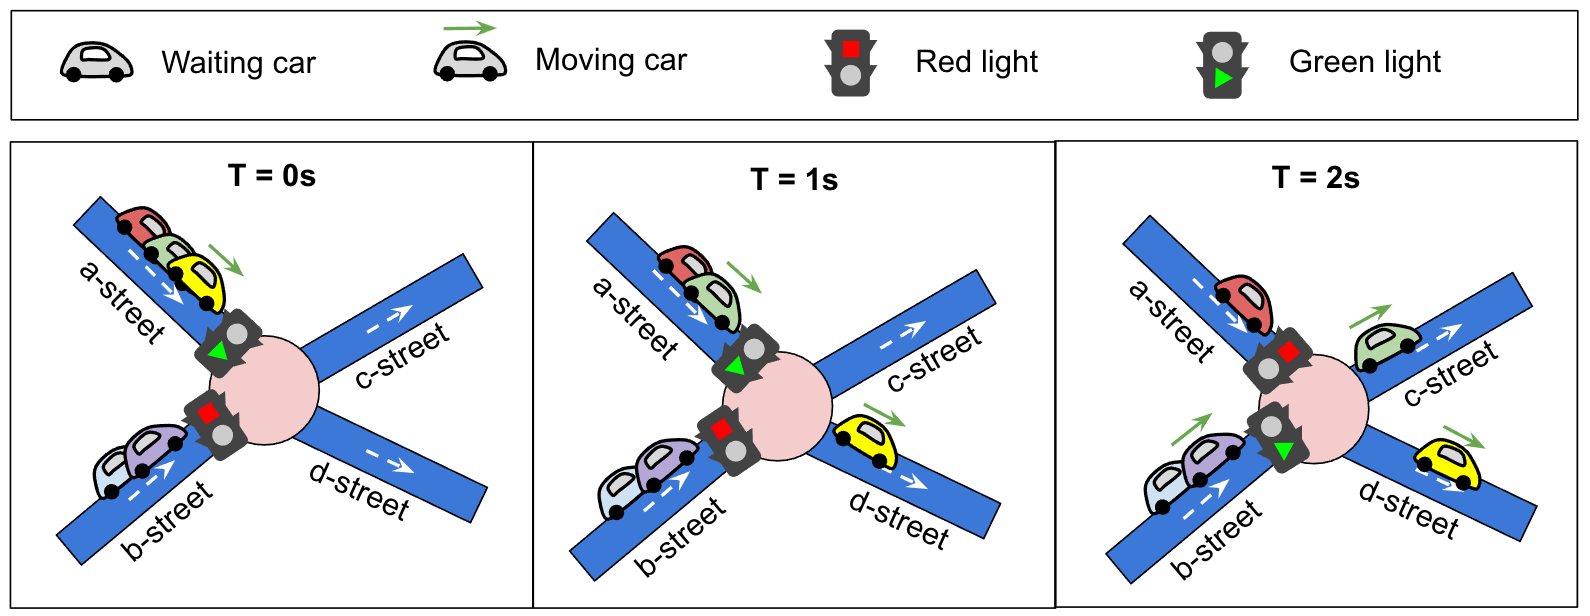
\includegraphics[width=\linewidth]{img/hashcode/figure2-abc.png}
    % 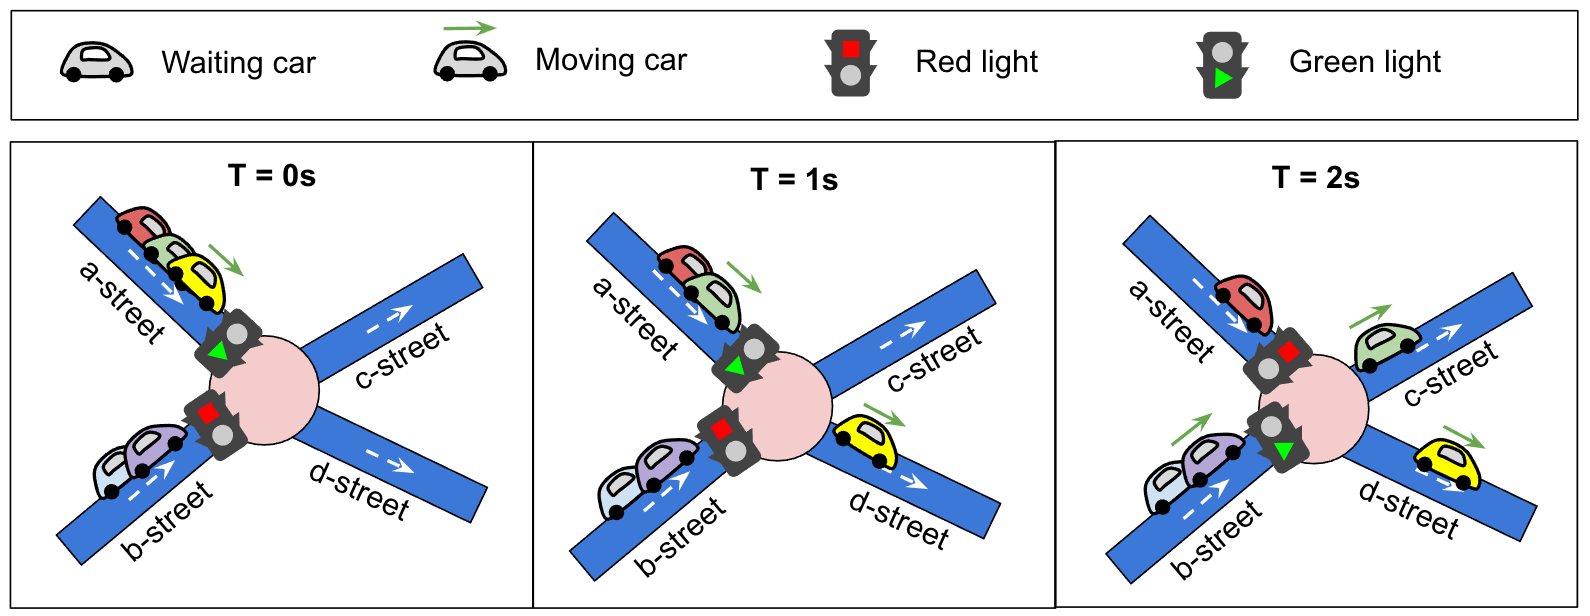
\includegraphics[width=.8\linewidth]{img/hashcode/figure2-abc.png}
    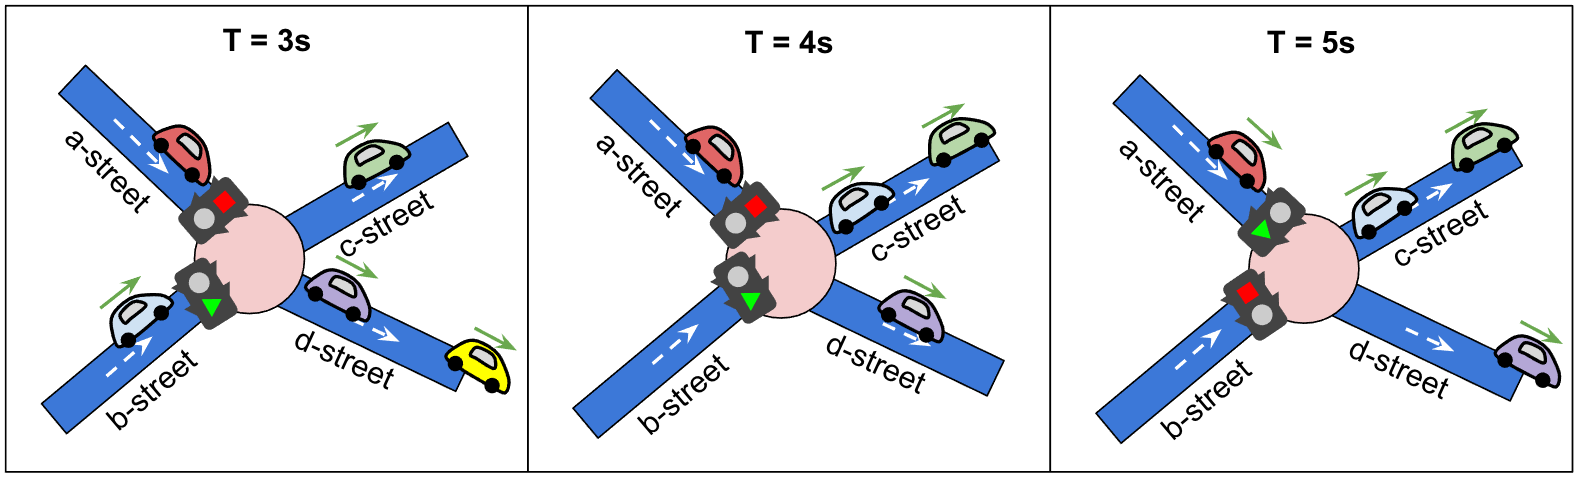
\includegraphics[width=\linewidth]{img/hashcode/figure2-def.png}
    % 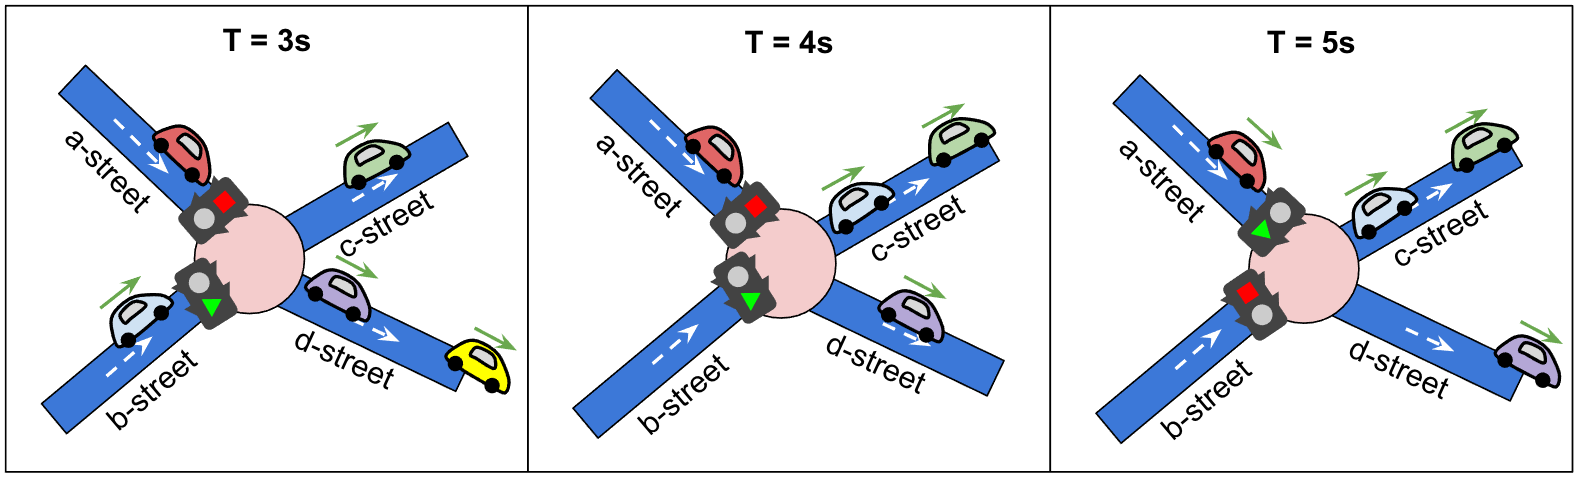
\includegraphics[width=.8\linewidth]{img/hashcode/figure2-def.png}
    \caption[Example of a traffic light schedule]{
        This figure shows how the traffic light schedule works for an intersection with two incoming streets \cite{google_coding_competitions}.
        The schedule is as follows: first \textit{a-street} for $2$ seconds, then \textit{b-street} for $3$ seconds.
        We can see that the first two cars from \textit{a-street} pass in the first two seconds, then the green light switches to \textit{b-street} for three seconds,
        letting the two cars from \textit{b-street} pass. The last car from \textit{a-street} waits till the beginning of the next cycle and then passes.
    }
    \label{fig:hashcode_traffic_lights}
\end{figure}

\subsection{Cars}

Dále máme množinu aut $C$, kde $1 \leq \abs{C} \leq 10^3$. Každé auto $c \in C$ má svou danou cestu městem, což je posloupnost ulic, kterými musí auto projet. Počet ulic v cestě je omezen --- $\forall c \in C \;\; 2 \leq \abs{\bm{p_c}} \leq 10^3$. V cestě se žádná křižovatka (tedy ani ulice) neopakuje.

Na začátku simulace se všechna auta nacházejí na konci první ulice své cesty, kde buď čekají na zelenou, nebo jsou připravena vyjet. Pokud se na konci nějaké ulice nachází více aut, jsou seřazena ve frontě v předem daném jednoznačném pořadí (see Figure~\ref{fig:hashcode_street}). Jakmile auto dorazí na konec poslední ulice své cesty, nečeká na zelenou ani se neřadí do fronty, ale je okamžitě odstraněno z ulice.

\begin{figure}[ht] % h = here, t = top, p = page of floats
    \centering
    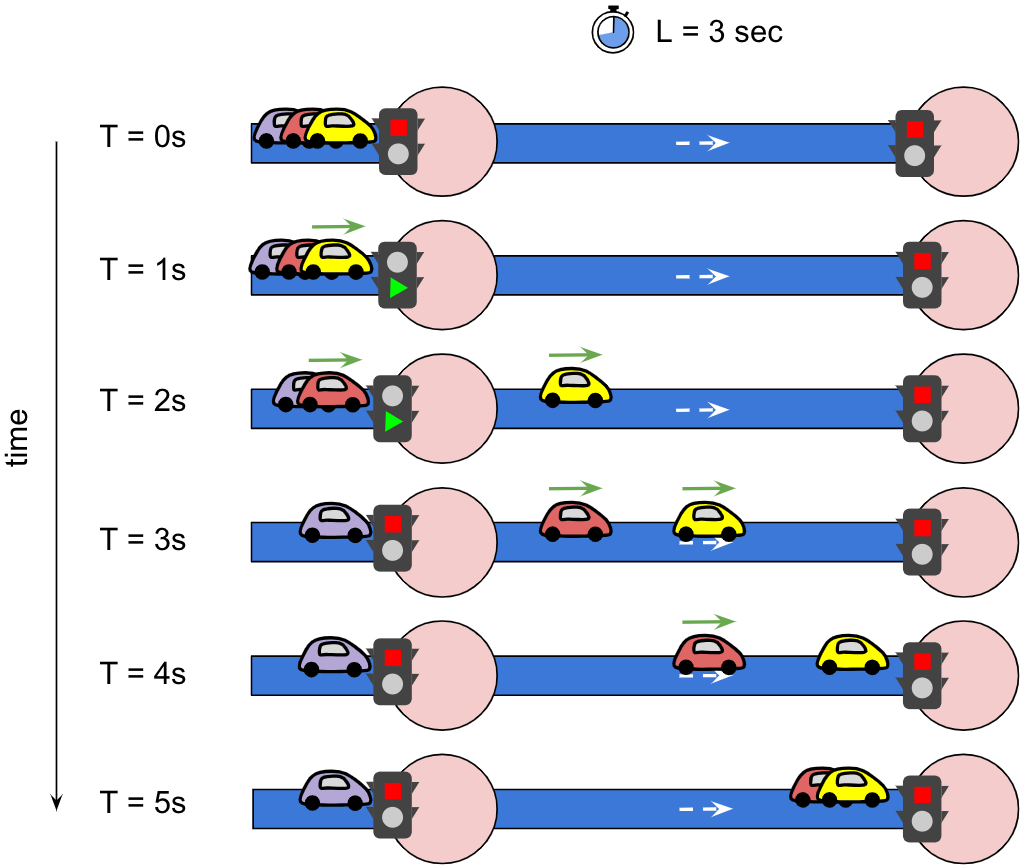
\includegraphics[width=\linewidth]{img/hashcode/figure3.png}
    %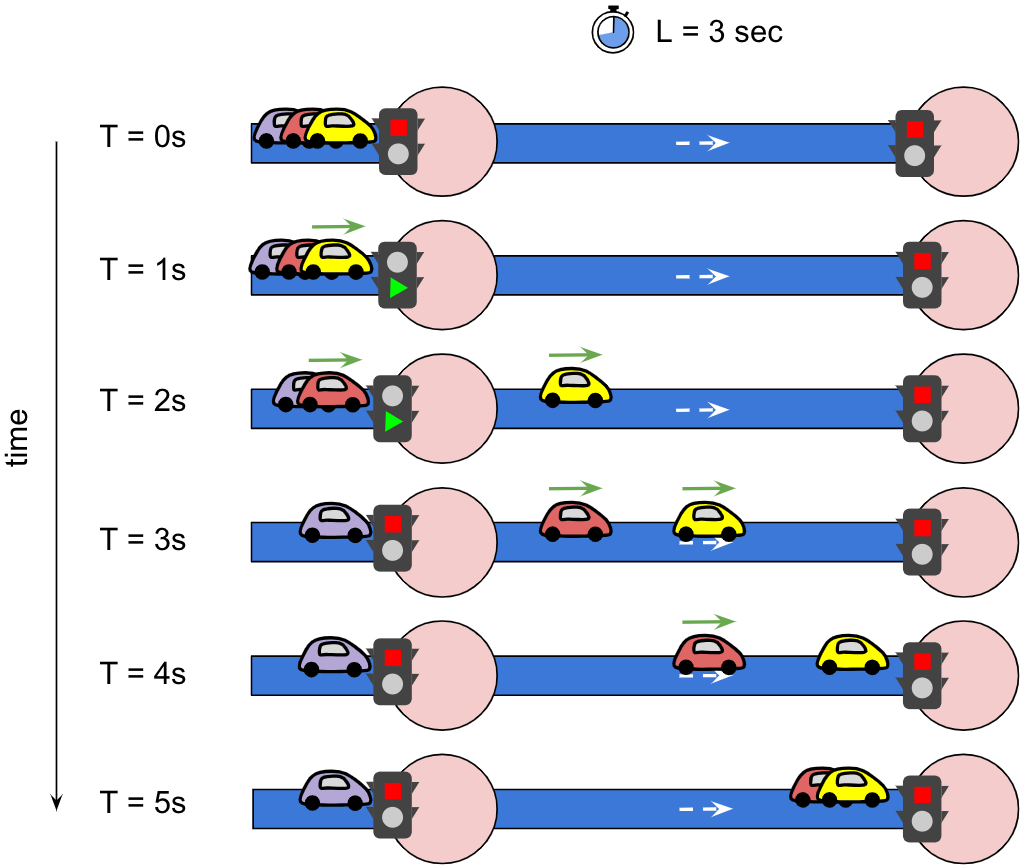
\includegraphics[width=.8\linewidth]{img/hashcode/figure3.png}
    \caption[Example of cars driving through a street]{
        This figure shows the first five seconds of a~simulation \cite{google_coding_competitions}.
        Note that for simplicity, only one street is shown in the figure; when the light is red for this street, it is green for another street in the same intersection.
        When the light turns green at $T=1s$, the first (yellow) car immediately passes the intersection and moves to the next street, reaching the end of the street at $T=4s$.
        At $T=2s$, the light is still green, so the second (red) car passes the intersection and moves to the next street, reaching the end of the street at $T=5s$.
        From $T=3s$ to $T=5s$, the light is red, so the third (purple) car cannot pass the intersection and has to wait for the next cycle.
    }
    \label{fig:hashcode_street}
\end{figure}

Skóre konkrétního nastavení plánů semaforů je určeno následovně: Máme danou délku trvání simulace $\mathrm{D}$ v sekundách, kde $1 \leq \mathrm{D} \leq 10^4$, a fixní bonus za dojetí auta do cílové destinace před koncem simulace $\mathrm{F}$, kde $1 \leq \mathrm{F} \leq 10^3$. Buď $t(c) \in \mathbb{N}$ čas, kdy auto $c \in C$ dorazí do cíle. Skóre auta $score(c)$ je definováno jako

\[
score(c) =
\begin{cases}
    \mathrm{F} + (\mathrm{D} - t(c)), & \text{if $t(c) \leq \mathrm{D}$}, \\
    0, & \text{otherwise}.
\end{cases}
\]

Pak celkové skóre řešení je definováno jako

\[
SCORE = \sum_{c \in C} score(c).
\]

%Let us start by describing the considered traffic signaling problem.
%It originally comes from the 2021 qualification round of Google Hash Code, which
%was a~global team programming competition. Teams of 2--4 individuals had to 
%solve a~programing challenge trying to achieve the best possible score in
%a~limited time window of 4 hours. Due to the format of the competition,
%the~participants mostly try to make a~simple working solution and then
%optimize it by changing values or running very simple heuristics. There is no time
%to try more sophisticated optimization methods.
%Also, only some of them are able to write a working simulator, which
%is necessary for the~real optimization of the problem.
%
%Unfortunatelly, Google shut down Hash Code together with other coding
%competitions in~2023. But the~problem statement\footnote{\url{https://github.com/google/coding-competitions-archive/blob/main/hashcode/hashcode_2021_qualification_round.pdf}}
%and~input data are still available in their Coding Competitions archive repository
%\cite{google_coding_competitions}.

%\section{Problem description}

%The following can be found in the original problem description in its entirety.
%Here, we provide a condensed version.
%In~short, the~task is this: \textit{Given a~city plan describing intersections and streets
%and~cars with planned paths throught the city, optimize the schedule of traffic
%lights to minimize the total amount of time spent in traffic, and~help as~many
%cars as~possible reach their final destination before a~specified deadline.}
%
%The city plan can be viewed as a~directed graph, where intersections are vertices
%and~streets are directed edges.

%\hfill\break
%\textbf{Intersection}
%\begin{itemize}
%    \item has at~least one incoming street and~at~least one outgoing street
%    \item When a~car crosses an intersection, note that it takes no extra time to move from the end of incoming street to the beginning of the outgoing street
%    \item May or may not have a~traffic light schedule
%\end{itemize}

%\hfill\break
%\textbf{Street}
%\begin{itemize}
%    \item Street is a~\textit{unique} connection between two intersections in one direction; separate streets in opposite directions between the same two intersections are possible though
%    \item has a fixed time $L$ it takes a~car to get from the~beginning to the~end of the~street independently of the~other cars on the~street
%\end{itemize}

%\hfil\break
%\textbf{Traffic light}
%\begin{itemize}
%    \item is at the~end of every street just before the~intersection
%    \item has two states: a~green light means the~cars from that street can cross the~intersection and head towards any other street; a~red light means the~cars from that street must stop and wait for green
%    \item At most one traffic light can be green at each intersection at any time
%    \item When the light is red, arriving cars queue up at the end of the street waiting for the light to turn green. When the light is green, one car can cross the intersection every second (see Figure~\ref{fig:hashcode_traffic_lights}). 
%\end{itemize}

%\hfil\break
%\textbf{Schedule}
%\begin{itemize}
%    \item The traffic light schedule sets the order and duration of green light for the incoming streets of the intersection (see Figure~\ref{fig:hashcode_traffic_lights})
%    \item The schedule keeps repeating in a cycle until the end of the simulation
%    \item Each street can appear \emph{at most once} in the schedule
%    \item Not all streets have to be included in the schedule --- those are always red
%    \item Intersections with no schedule are always red for all incoming streets
%\end{itemize}

%\hfill\break
%\textbf{Car}
%\begin{itemize}
%    \item Each cars has its own path --- a~sequence of streets it drives through
%    \item Each path goes through any intersection at most once --- cycles are not allowed
%    \item At the beginning of the simulation, all cars start at the end of the first street in their path, waiting for the green light, or ready to move if the light is green
%    \item If more cars start at the~end of the same street, they queue up in the order they appear in the input (see Figure~\ref{fig:hashcode_street})
%    \item When a~car reaches the end of the last street in its path, it is immediately removed from the street --- it does not wait for the green light and does not take space in the queue
%\end{itemize}

%\hfill\break
%\textbf{Score}
%\begin{itemize}
%    \item The traffic light schedules are evaluated by the following scoring function: Given a duration of the simulation $D$ and a fixed bonus for reaching the destination $F$, a~car finishing its path at time $T$ receives the following $score$: 
%\end{itemize}
%
%\[
%score(c) =
%\begin{cases}
%    F + (D - T), & \text{if $T \leq D$}, \\
%    0, & \text{otherwise}.
%\end{cases}
%\]
%
%Then the total score of the solution is the~sum of the~scores of all cars.

